\begin{table*}[t]
  \captionof{table}{DFiant Hierarchy Example: Inheritance, Polymorphism, Recursive Composition, and Inlined View}
  \label{tbl:Box}
  \begin{tabular}{|c|c|c|}
    \hline 
    \textbf{Description} & \textbf{DFiant Code} & \textbf{Functional Drawing} \\ 
    \hline
    \begin{minipage}{0.1\textwidth}
      \footnotesize
      \flushleft
      Abstract base class, \code{Box} (defines only an interface)
    \end{minipage} 
    &
    \begin{minipage}{0.48\textwidth}
      \begin{minted}[autogobble,tabsize=2,framesep=1pt,fontsize=\fontsize{8}{8}\selectfont]{scala}
      type DFB = DFUInt[32] //Type alias, to save code space
      abstract class Box(iT: DFB, iB: DFB) { //T=Top, B=Bottom 
        val oT: DFB
        val oB: DFB
      }
      \end{minted}
    \end{minipage} 
    &  
    \begin{minipage}[c][1.5cm]{0.34\textwidth}
      \centering
      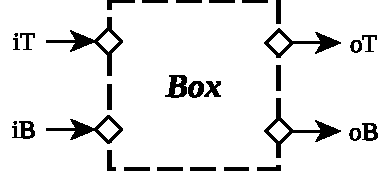
\includegraphics[height=1.3cm]{graphics/Box.pdf}%
    \end{minipage} 
    \\ 
    \hline 
    \begin{minipage}{0.1\textwidth}
      \footnotesize
      \flushleft
      Concrete \code{Box} implementation examples
    \end{minipage} 
    &
    \begin{minipage}{0.48\textwidth}
      \begin{minted}[autogobble,tabsize=2,framesep=1pt,fontsize=\fontsize{8}{8}\selectfont]{scala}
      case class BoxY(iT: DFB, iB: DFB) extends Box(iT, iB) {
        val (oT, oB) = (iT * iT, iT + iB)
      }
      case class BoxE(iT: DFB, iB: DFB) extends Box(iT, iB) {
        val (oT, oB) = (iT + iB, iB)
      }
      \end{minted}
    \end{minipage} 
    &  
    \begin{minipage}[c][1.8cm]{0.34\textwidth}
      \centering
      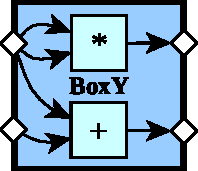
\includegraphics[height=1.3cm]{graphics/BoxY.pdf}%
      \quad\quad\quad
      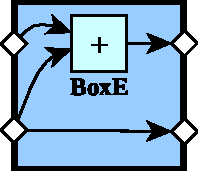
\includegraphics[height=1.3cm]{graphics/BoxE.pdf}%
    \end{minipage} 
    \\ 
    \hline
    \begin{minipage}{0.1\textwidth}
      \footnotesize
      \flushleft
      \code{Box123}, an abstract polymorphic composition of three \code{Box} instances
    \end{minipage} 
    &
    \begin{minipage}{0.48\textwidth}
      \begin{minted}[autogobble,tabsize=2,framesep=1pt,fontsize=\fontsize{8}{8}\selectfont]{scala}
      abstract class Box123(iT: DFB, iB: DFB) extends Box(iT, iB){
        def b1Bld(iT: DFB, iB: DFB) : Box
        def b3Bld(iT: DFB, iB: DFB) : Box
        val b1 = b1Bld(iT,     iB)
        val b2 = BoxE(b1.oB,   b1.oT)
        val b3 = b3Bld(b2.oB,  b2.oT)
        val (oT, oB) = (b3.oT, b3.oB)
      }
      \end{minted}
    \end{minipage} 
    &  
    \begin{minipage}[c][2.3cm]{0.34\textwidth}
      \centering
      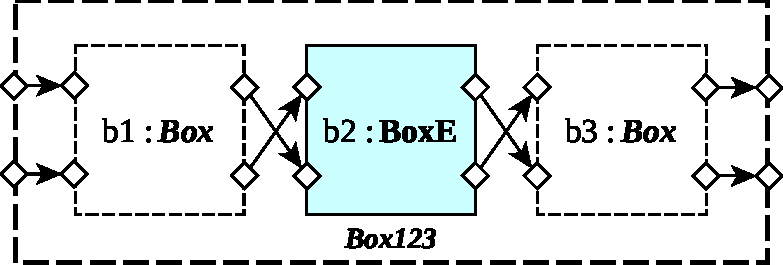
\includegraphics[height=2.1cm]{graphics/Box123.pdf}%
    \end{minipage} 
    \\ 
    \hline
    \begin{minipage}{0.1\textwidth}
      \footnotesize
      \flushleft
      \code{BoxYEE}, a concrete polymorphic composition of three \code{Box} instances \\+\\An inlined view of \code{BoxYEE}
    \end{minipage} 
    &
    \begin{minipage}{0.48\textwidth}
      \begin{minted}[autogobble,tabsize=2,framesep=1pt,fontsize=\fontsize{8}{8}\selectfont]{scala}
      case class BoxYEE(iT: DFB, iB: DFB) extends Box123(iT, iB) {
        def b1Bld(iT: DFB, iB: DFB) = BoxY(iT, iB)
        def b3Bld(iT: DFB, iB: DFB) = BoxE(iT, iB)
      }
      \end{minted}
    \end{minipage} 
    &  
    \begin{minipage}[c][4.6cm]{0.34\textwidth}
      \centering
      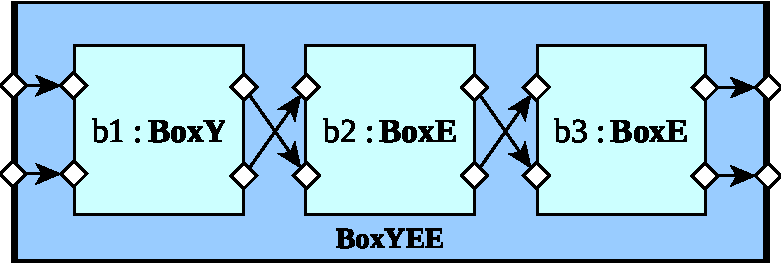
\includegraphics[height=2.1cm]{graphics/BoxYEE.pdf} \\
      \vspace{0.1cm}
      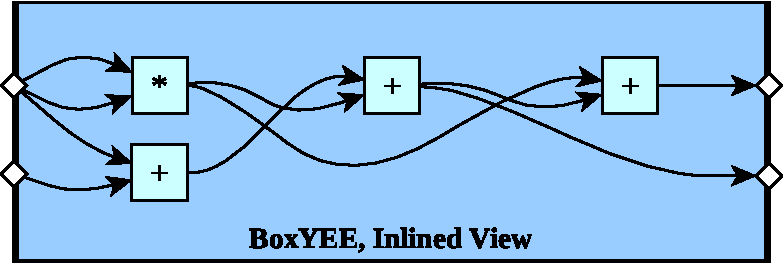
\includegraphics[height=2.1cm]{graphics/BoxYEEInlined.pdf}%
    \end{minipage} 
    \\ 
    \hline
    \begin{minipage}{0.1\textwidth}
      \footnotesize
      \flushleft
      Finite recursive composition example
    \end{minipage} 
    &
    \begin{minipage}{0.48\textwidth}
      \begin{minted}[autogobble,tabsize=2,framesep=1pt,fontsize=\fontsize{8}{8}\selectfont]{scala}
      case class BoxBox(N: Int)(iT: DFB, iB: DFB) 
      extends Box(iT, iB) {
        val b = BoxY(iT, iB)
        val bb : Box = if (N > 0) BoxBox(N - 1)(b.oT, b.oB)
                       else b
        val (oT, oB) = (bb.oT, bb.oB)
      }
      \end{minted}
    \end{minipage} 
    &  
    \begin{minipage}[c][2.3cm]{0.34\textwidth}
      \centering
      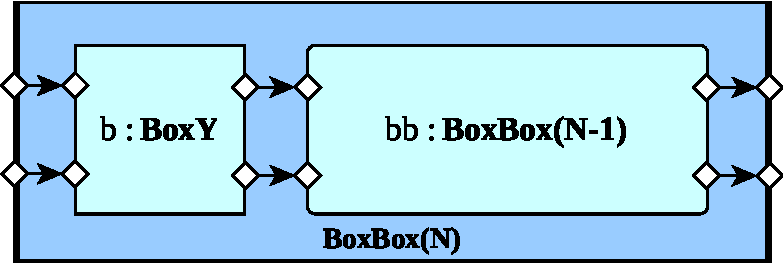
\includegraphics[height=2.1cm]{graphics/BoxBox.pdf}%
    \end{minipage} 
    \\ 
    \hline
  \end{tabular} 
\end{table*}
